\documentclass[11pt]{article}
\usepackage{naacl2012}
\usepackage{times}
\usepackage{latexsym}
\usepackage{amsmath}
\usepackage{algorithm}
\usepackage{algorithmic}
\usepackage{multirow}
\usepackage{url}
\usepackage{graphicx} 
\usepackage{longtable}
\usepackage{caption}

\DeclareMathOperator*{\argmax}{arg\,max}
%\setlength\titlebox{6.5cm}
\setlength\titlebox{2.7cm}

\title{Experiments: Phrase-based MT + Bilingual Lexicon Induction}
\author{Ann Irvine and Chris Callison-Burch}

\begin{document}

\maketitle

\section{Introduction}
This technical report describes three sets of experiments which are related to low resource machine translation. The first set evaluates a bilingual lexicon induction technique and the second two supplement a phrase-based MT system with scores and translations based on bilingual lexicon induction.

We first evaluate the performance of a Rapp-style \cite{Rapp:1995} bilingual lexicon induction framework. We use monolingual web crawl and wikipedia data to rank candidate translations for a given source language word. We perform experiments identifying English translations for words in {\it 23} source languages. We evaluate our results against dictionaries compiled using Mechanical Turk. 

We then supplement a phase-based MT system \cite{moses} with the scores and translations that are the output of our bilingual lexicon induction framework. We use our assumed dictionaries, scores based on monolingual data, and induced translations to translate the same five Wikipedia pages for each of our 24 languages of interest. Because clean machine translation test sets do not exist for every language on our list, we do a qualitative analysis of the outputs.

In our third set of experiments, we evaluate our techniques in the standard way, using an MT test set and measuring performance with the BLEU metric. In these experiments, we vary the amount of training data that we use to train the model. We also compare systems based only on parallel sentences with those which also access dictionaries and induced translations for OOV unigrams.


%\section{Background}
%\subsection{Phrase-Based SMT}
%\subsection{Low Resource MT}
%\subsection{Lexicon Induction}

\section{Data}
\subsection{Monolingual data}
{\bf Web crawls} We have crawled online news websites for monolingual data in many of the world's languages. We used language-labeled Wikipedia data to train a language classifier. Because our data is comprised of news stories, each document also has an associated time stamp, which turns out to be useful (see Section \ref{ssec:temporal}). The amount of data that we have gathered for each of our 24 languages of interest is shown in Table \ref{table:crawls}.

\begin{table}\footnotesize
\begin{center}
\begin{tabular}{|l|c|l|c|}
\hline
\multirow{2}{*}{Language} & Thousands of & \multirow{2}{*}{Language} & Thousands of \\
&word tokens&&word tokens\\
\hline
%Malaysian & $57$ & Azeri & $124$ \\
Azeri & $124$ & Nepali & $127$ \\
Tamil & $189$ & Somali & $451$ \\
Uzbek & $627$ & Romanian & $2,867$ \\
Albanian & $3,313$ & Indonesian & $3,841$ \\
Welsh & $3,922$ & Bengali & $4,033$ \\
Serbian & $5,694$ & Bosnian & $7,354$ \\
Polish & $7,832$ & Turkish & $9,089$ \\
Ukrainian & $15,171$ & Bulgarian & $30,543$\\
Latvian & $35,098$ & Hindi & $42,111$ \\
Slovak & $109,335$ & Urdu & $284,725$\\
Farsi & $697,706$ & Spanish & $783,093$ \\
Russian & $1,515,036$ & &\\
\hline
\end{tabular}
\end{center}
%\vskip -0.1in
\caption{\label{table:crawls}Amount of monolingual online news crawls data, by language.}
%\vskip -0.15in
\end{table}


{\bf Wikipedia} In addition to our data from web crawls, we also use Wikipedia as a source of monolingual data. To maximize the degree of comparability between our source language Wikipedia pages and English Wikipedia, we only use those pages which have interlingual links with English pages. The amount of Wikipedia data that we use for each language is given in Table \ref{table:wiki}.

\begin{table}\footnotesize
\begin{center}
\begin{tabular}{|l|c|l|c|}
\hline
\multirow{2}{*}{Language} & Thousands of & \multirow{2}{*}{Language} & Thousands of \\
&word tokens&&word tokens\\
\hline
Azeri & $2,518$ & Nepali & $262$ \\
Tamil & $3,484$ & Somali & $82$\\
Uzbek & $747$ & Romanian & $21,157$ \\
Albanian & $3,197$ & Indonesian & $18,021$ \\
Welsh & $3,592$ & Bengali & $2,607$ \\
Serbian & $20,083$ & Bosnian & $5,457$ \\
Polish & $96,739$ & Turkish & $22,080$ \\
Ukrainian & $22,383$ & Bulgarian & $19,045$\\
Latvian & $5,064$ & Hindi & $5,349$\\
Slovak & $15,341$ & Urdu & $2,163$\\
Farsi & $12,291$ & Spanish & $189,171$\\
Russian & $105,084$ & &\\
\hline
\end{tabular}
\end{center}
%\vskip -0.1in
\caption{\label{table:wiki}Amount of Wikipedia data, by language.}
%\vskip -0.15in
\end{table}

\subsection {Dictionaries}\label{ssec:dicts}

Throughout the experiments we use two different sets of dictionaries. The first comes from a large collection of dictionaries, gathered from a variety of sources. Some were originally paper dictionaries which have been OCR'd. Others were originally electronic dictionaries. For some languages, we have multiple dictionaries, and we have simply concatenated them for the experiments described here. Some dictionaries only contain unigram translations while others contain translations of some source language phrases. These dictionaries will henceforth be referred to as the {\it standard dictionaries}. 

We also use a set of dictionaries that were created using Mechanical Turk. In that dictionary creation, source language words were chosen starting with the most frequent words in that language's Wikipedia \footnote{Is that true?}. Although all of the source words in the Wikipedia dictionaries are unigrams, we allowed workers to translate them into multi-word English phrases. 

Both the standard dictionaries and the MTurk dictionaries are described in Table \ref{table:dicts}.

\begin{table*}\footnotesize
\begin{center}
\begin{tabular}{|l||c|c|c||c|c||c|}
\hline
\multirow{2}{*}{Language} & \multicolumn{3}{|c||}{Standard dictionary} & \multicolumn{2}{|c||}{MTurk dictionary} & \multirow{2}{*}{Script}\\ \cline{2-6}
& Source words &Translations & Dict Source & Source words & Translations & \\
%Language & Src Tokens & Translations & Dict Source(s) \\
\hline
Azeri  & $227,727$ & $231,891$ &  e+o & $7,814$ & $8,121$ & r \\
Nepali  & $4,770$ & $6,812$ &  o & $12,314$ & $17,752$ & d \\
Tamil  & $58,236$ & $165,004$ &   e  & $9,146$ & $14,551$ & o \\
Somali  & $227$ & $230$ &   e & $9,881$ & $11,157$ & r \\
Uzbek  & $124,989$ & $190,688$ & e+o & $5,163$ & $6,710$ & r \\
Romanian  & $48,088$ & $249,479$ &  e & $9,131$ & $12,362$ & r \\
Albanian  & $44,245$ & $188,563$ &  e  & $9,736$ & $12,041$ & r\\
Indonesian  & $32,311$ &  $67,633$ & e+o & $9,236$ & $12,594$ & r\\
Welsh  & $14,586$ &  $25,832$ &   e & $9,013$ & $9,357$ & r\\
Bengali  & $1,481$ & $1,606$   & e & $9,461$ & $14,777$ & o \\
Serbian  &  $55,349$ & $168,140$ & e & $9,622$ & $13,511$ & c\\
Bosnian    & $9,641$ & $18,283$ & o & $9,681$ & $13,366$ & r\\
Polish  & $56,233$ &  $261,463$ &   e & $9,467$ &  $13,725$ & r\\
Turkish  & $488,738$ &  $1,272,881$  & e+o & $9,403$ &  $13,686$ & r \\
Ukrainian    & $8,324$ & $14,056$ &  e   & $8,119$ & $8,533$ & c\\
Bulgarian  & $72,720$ & $316,631$ &  e  & $9,607$ &  $12,442$ & c \\
Latvian  & $33,486$ & $148,363$ &   e & $8,624$ &  $9,896$ & r \\
Hindi  & $25,305$ & $58,179$ &   e & $8,014$ & $10,721$ & d\\
Slovak  & $48,683$ & $233,093$   & e  & $9,495$ & $11,998$ & r \\
Urdu  & $24,271$ &  $113,911$  & e & $8,088$ & $11,254$ & a \\
Farsi  & $101,620$ &  $198,605$  &  e+o & $1,845$ & $1,970$ & a \\
Spanish  &  $73,589$  & $347,441$ & e  & $8,970$ & $11,566$ & r \\
Russian  & $89,785$ & $423,009$ & e & $9,188$ & $11,785$ & c \\
\hline
\end{tabular}
\end{center}
%\vskip -0.1in
\caption{\label{table:dicts}Description of both standard and MTurk dictionaries. The number of unique source words and phrases in each dictionary is given along with the total number of translations. The source(s) of each standard dictionary is also given. {\it e} indicates that a dictionary was originally electronic and {\it o} indicates a paper dictionary that have been OCR'd. In some cases, we have both types of dictionaries for a given language. The final column indicates whether the primary script used in our dictionaries (as well as monolingual datasets) is Roman (r), Cyrillic (c), Arabic (a), Devanagari (d), or other (o).}
%\vskip -0.15in
\end{table*}

\subsection{Languages}
We chose the 23 languages listed because, for each, we had access to standard and MTurk dictionaries as well as some monolingual data from both the web crawls and Wikipedia. Additionally, we included some truly low resource languages (e.g. Somali, Nepali) and also some high resource languages for which we could more thoroughly evaluate MT performance (e.g. Urdu, Spanish).

\section{Experiments 1: Bilingual lexicon induction}\label{sec:lexinduc}
In our first set of experiments, we evaluate the quality of a bilingual lexicon induction framework that combines monolingual distributional, temporal, and orthographic signals to rank target language word translations for a given source language unigram. 

\subsection{Contextual Similarity} 
We score monolingual distributional similarity by first collecting contextual vectors for each source and target language unigram. The contextual vector for a given source language word, $w_{s_i}$, is the size of the source language vocabulary, $|V_s|$, and contains counts of how many times each word in the source language vocabulary appeared in the context of word $w_{s_i}$. In the experiments presented here, we use bag of words contexts in a window of size two (two words to the left of $w_{s_i}$ and two words to the right). Similarly, we collect context vectors for all target language words, $w_{t_j}$. In all experiments, we use the MTurk dictionaries to project the target language contextual vectors into the source language feature space in order to keep the dictionary size and quality constant across all source languages. Since the dictionaries are of reasonable size (see Table \ref{table:dicts}), we expect the quality of the projections to be sufficient for the task. We gather both source and target language contextual vectors from our web crawl data.

\subsection{Temporal Similarity}\label{ssec:temporal}
We gather temporal signatures for each source and target language unigram from our time-stamped web crawl data. That is, temporal signatures for a given word contain counts corresponding to how many times that word appeared in news articles with a certain date. We expect that source and target language words which are translations of one another will appear with similar frequencies over time in monolingual data. We collect temporal signatures over dates for which we have monolingual data in both languages. Our English web crawl data is essentially limitless, so we restrict the English data that we use in a particular source language experiment to be no more than three times the size of our source language web crawled data, and only include news articles from those dates for which we also have source language articles.

\subsection{Orthographic Similarity} 
We measure orthographic similarity between a pair of words as the normalized\footnote{Normalized by the average of the lengths of the two words} edit distance between the two words. We expect the edit distance between an English word and a word from a source language which is also written in the roman script to be quite informative, particularly for word classes that tend to be transliterated, rather than translated, across languages (e.g. person and place names). In these experiments, we do not first transliterate non-roman script source language words before computing edit distance. Thus, for non-roman source languages, none of the characters will match, and our edit distance measure is simply an indication of the difference in length between the two words. 

\subsection{Score Aggregation} 
Rather than using absolute scores, we aggregate the {\it ranked lists} provided by each of the above three similarity measures. That is, for a given source language word, we score and rank all target language candidate translations (the target language vocabulary) using each of the above three metrics. We then compute the {\it mean reciprocal rank} (MRR) for each target language word and produce a new ranking based on the MRRs.

\subsection{Results}
For each source language, we evaluate the above bilingual lexicon induction framework using percent accuracy in the top-1, top-10, and top-100 ranked target language word lists, compared against the MTurk dictionaries. This measure is somewhat conservative since the MTurk dictionaries aren't expected to be exhaustive, meaning that some target language translations for a given source language word won't appear in the dictionary and the system won't be given credit for ranking these target items high in its translation list. For each source language word, the target language list of candidate translations contains all unique word types observed in our target language monolingual corpus (in the case of these experiments, English web crawl data). 

Figures \ref{fig:bli.az} through \ref{fig:bli.sk} present the bilingual lexicon induction experimental results. In each experiment, the $3,000$ most frequent source language words in the MTurk dictionary, with respect to the monolingual crawls data, were divided into 10 bins, by frequency. That is, the most frequent 300 source language words were put in the first bin, and the least frequent (among the most frequent 3000) 300 source language words were put into the tenth bin. The horizontal access in each figure plots the average corpus frequency of the words in a given bin versus the percent of those 300 source language words that have a correct translation in the top-k ranked list of translations. In general, our monolingual signals are stronger for those words that appear frequently in monolingual corpora than for those words that appear less frequently and have sparse context and temporal counts. Therefore, translation accuracy tends to be higher for frequent words than for less frequent words, resulting in accuracies that go up from left to right, or from lower frequency to higher frequency, in the figures.
 
The results are presented starting with the language with the least amount of monolingual web crawl data (Azeri, Figure \ref{fig:bli.az}) and ending with the language with the largest amount of monolingual web crawl data (Slovak, Figure \ref{fig:bli.sk}). Corpus frequencies for even the most frequent words in the first few source languages are very small. For example, the average frequency of the 300 most frequent Azeri and Nepali words is around 200. For those languages which we have very little monolingual data, all of the contextual and temporal vectors are sparse and translation accuracies are low.

As we have access to more monolingual data, the figures look more regular. That is, given a sufficient amount of monolingual text, we do observe that our translation accuracy is higher for more frequent source language words than for less frequent source language words. This trend is particularly clear in the Albanian (Figure \ref{fig:bli.sq}) and Indonesian (Figure \ref{fig:bli.id}) plots.

Performance among Indian languages, including Nepali, Hindi, Bengali, and Tamil, is particularly low. While we have collected very small amounts of Nepali and Tamil web crawl monolingual data, the amount of Bengali data is modest, and we have a large amount of Hindi data. Yet, top-100 accuracy for even the most frequent Hindi words is only around 15\%. We suspect that adding transliteration-based edit distance scores will boost performance somewhat. It is also possible that English and Indian language news articles are less comparable than other language pairs. 

We see the highest accuracies for Albanian, Indonesian, and Romanian. Performance for Bosnian, Polish, and Welsh is also not bad. All six of these languages, like English, are written in the roman script, and we suspect that the edit distance similarity metric is able to capture a lot of transliterations and cognates. 

\subsection{Future Work}
Our immediate plans for future work are the following:
\begin{enumerate}
\item{Incorporate a transliteration module that will enable high-quality edit distance scoring for source languages written in all scripts.}
\item{Also use Wikipedia monolingual data to induce bilingual lexicons.}
\end{enumerate}



\begin{figure}[h]
%\vskip 0.0in
\begin{center}
\includegraphics[width=0.9 \linewidth]{../byFreqGraphs/az/lexinductnew.pdf}
\vskip -0.15in
\caption{Azeri bilingual lexicon induction results}
%\vskip -0.2in
\label{fig:bli.az} 
\end{center}
\end{figure}

\begin{figure}[h]
%\vskip 0.0in
\begin{center}
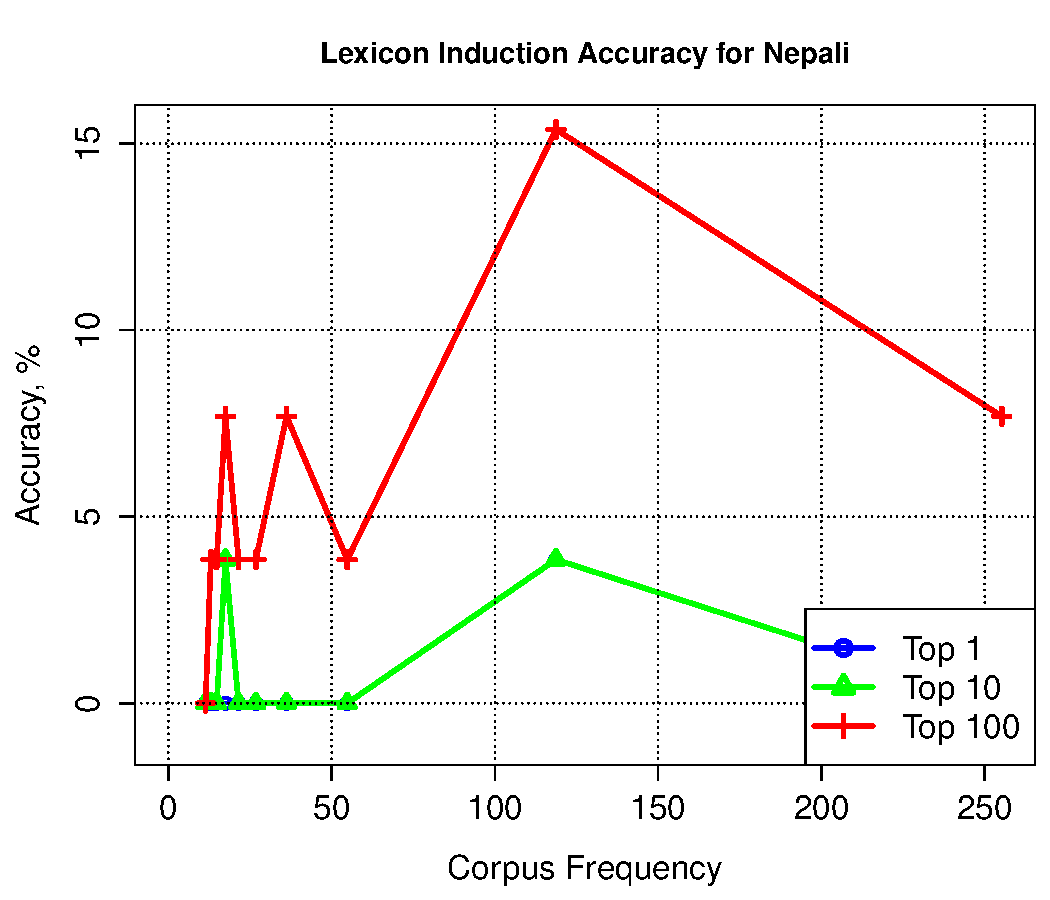
\includegraphics[width=0.9 \linewidth]{../byFreqGraphs/ne/lexinductnew.pdf}
\vskip -0.15in
\caption{Nepali bilingual lexicon induction results}
%\vskip -0.2in
\label{fig:bli.ne} 
\end{center}
\end{figure}

\begin{figure}
%\vskip 0.0in
\begin{center}
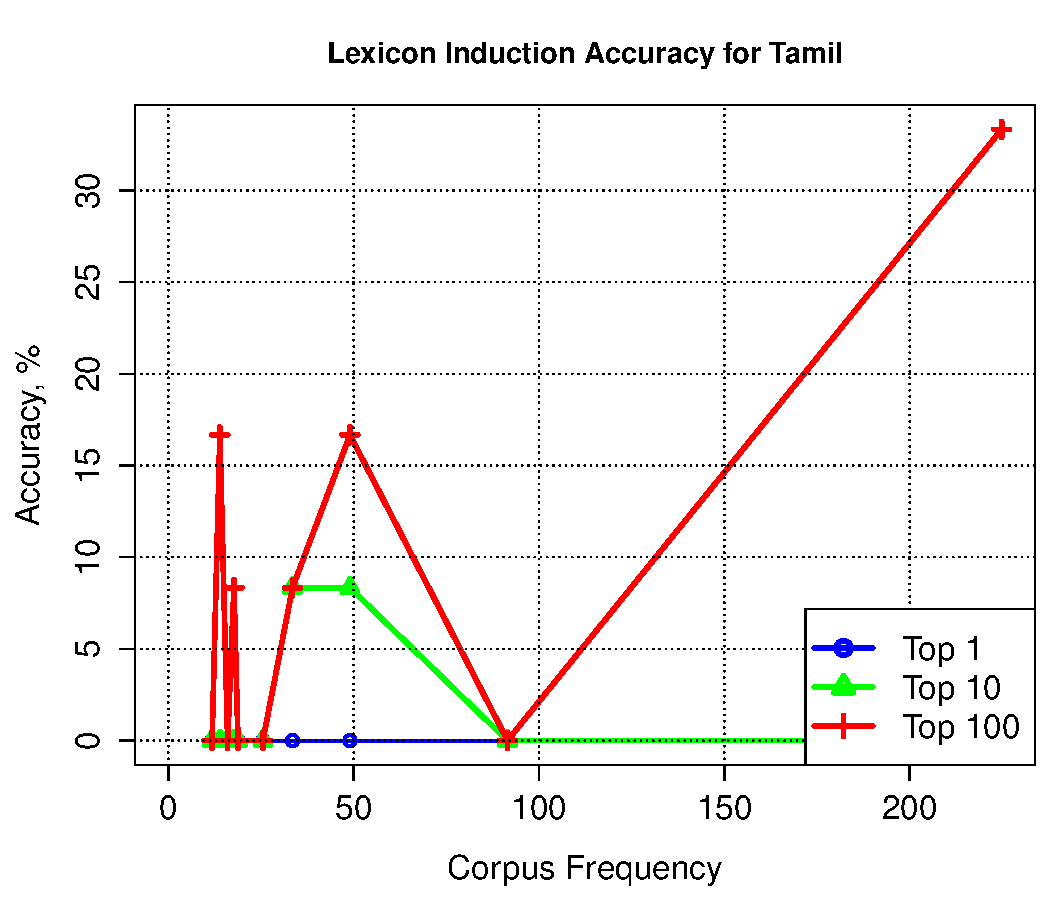
\includegraphics[width=0.9 \linewidth]{../byFreqGraphs/ta/lexinductnew.pdf}
\vskip -0.15in
\caption{Tamil bilingual lexicon induction results}
%\vskip -0.2in
\label{fig:bli.ta} 
\end{center}
\end{figure}

\begin{figure}
%\vskip 0.0in
\begin{center}
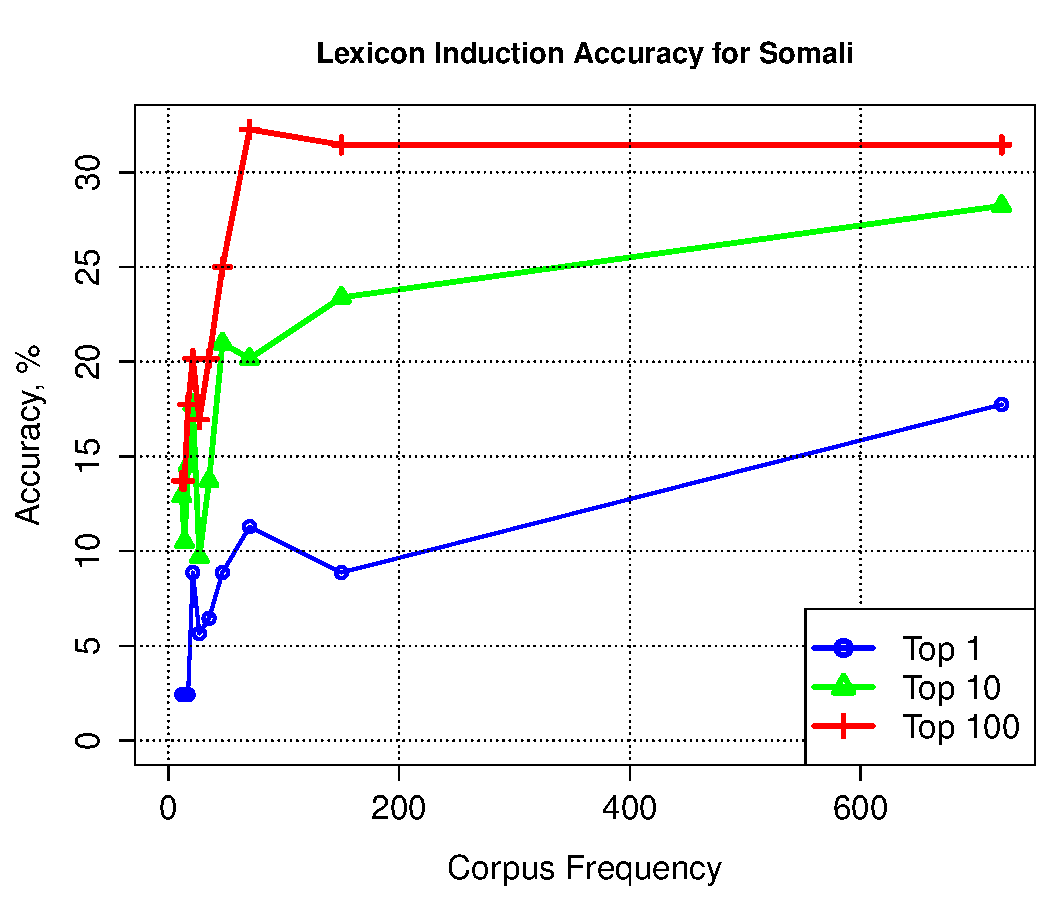
\includegraphics[width=0.9 \linewidth]{../byFreqGraphs/so/lexinductnew.pdf}
\vskip -0.15in
\caption{Somali bilingual lexicon induction results}
%\vskip -0.2in
\label{fig:bli.so} 
\end{center}
\end{figure}

\begin{figure}
%\vskip 0.0in
\begin{center}
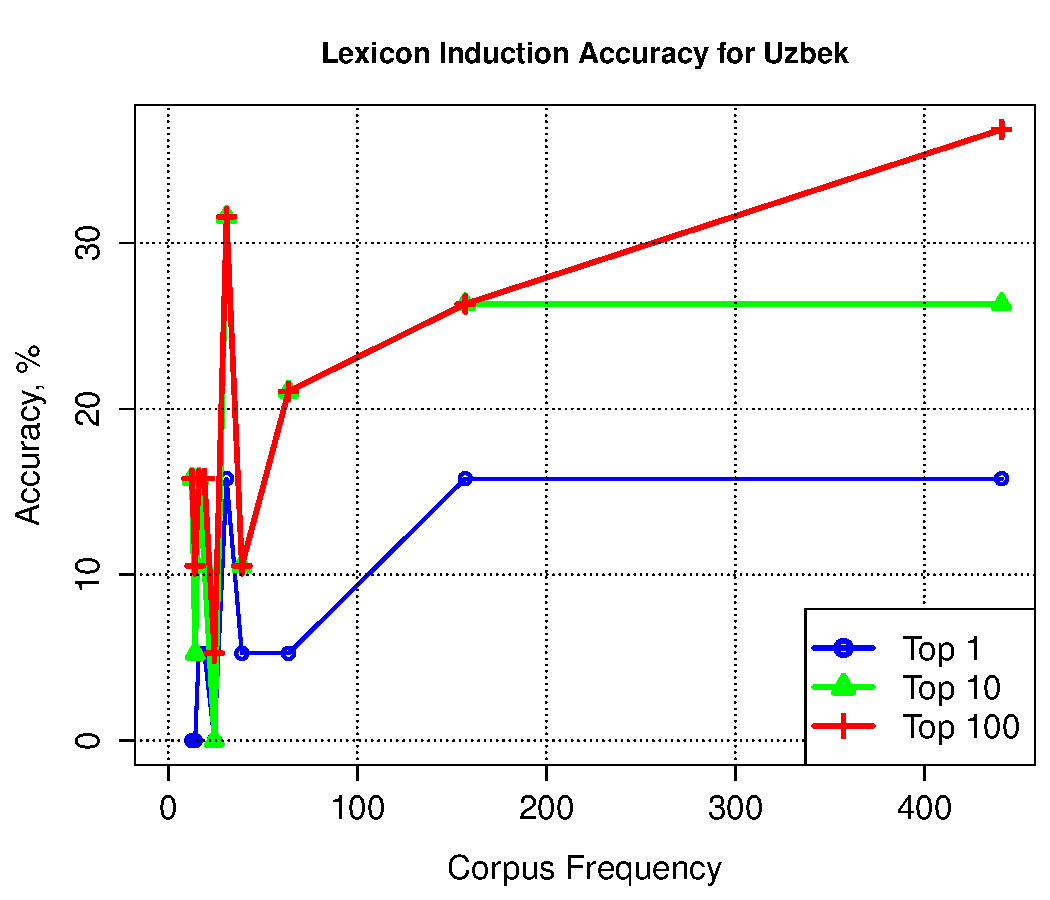
\includegraphics[width=0.9 \linewidth]{../byFreqGraphs/uz/lexinductnew.pdf}
\vskip -0.15in
\caption{Uzbek bilingual lexicon induction results}
%\vskip -0.2in
\label{fig:bli.uz} 
\end{center}
\end{figure}

\begin{figure}
%\vskip 0.0in
\begin{center}
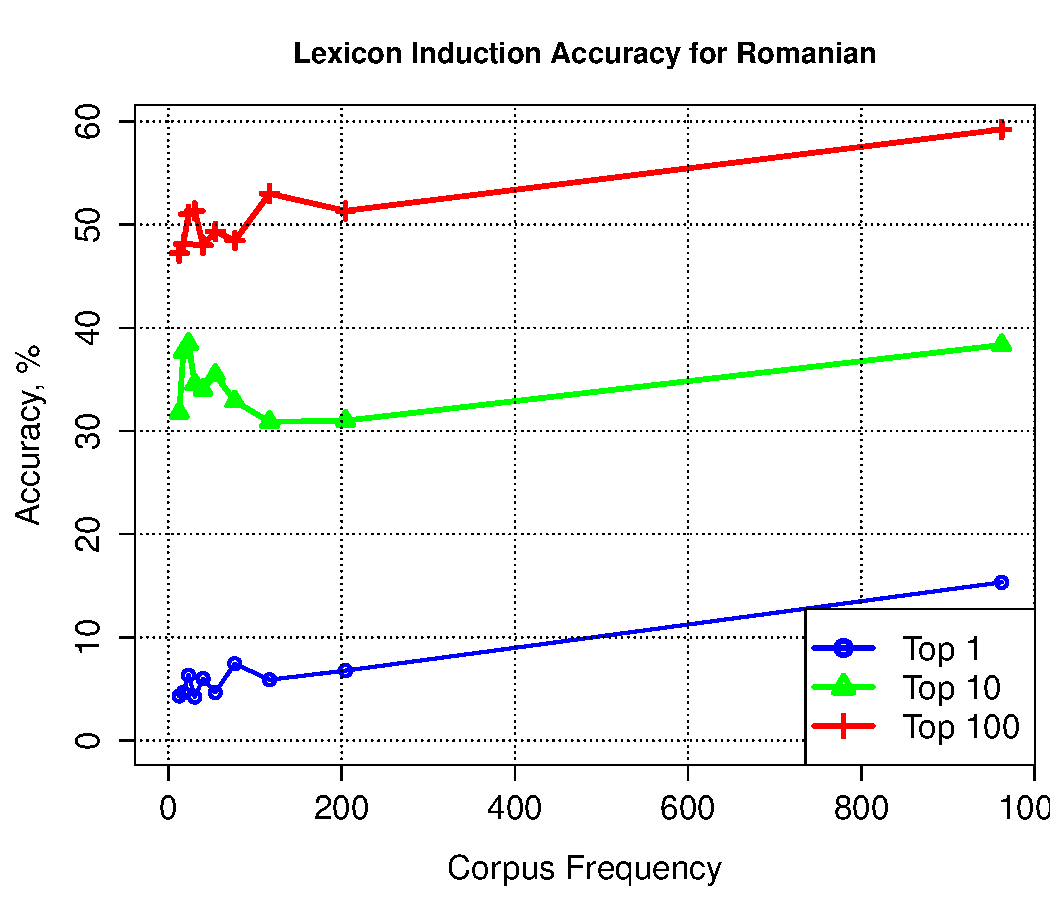
\includegraphics[width=0.9 \linewidth]{../byFreqGraphs/ro/lexinductnew.pdf}
\vskip -0.15in
\caption{Romanian bilingual lexicon induction results}
%\vskip -0.2in
\label{fig:bli.ro} 
\end{center}
\end{figure}



\begin{figure}
%\vskip 0.0in
\begin{center}
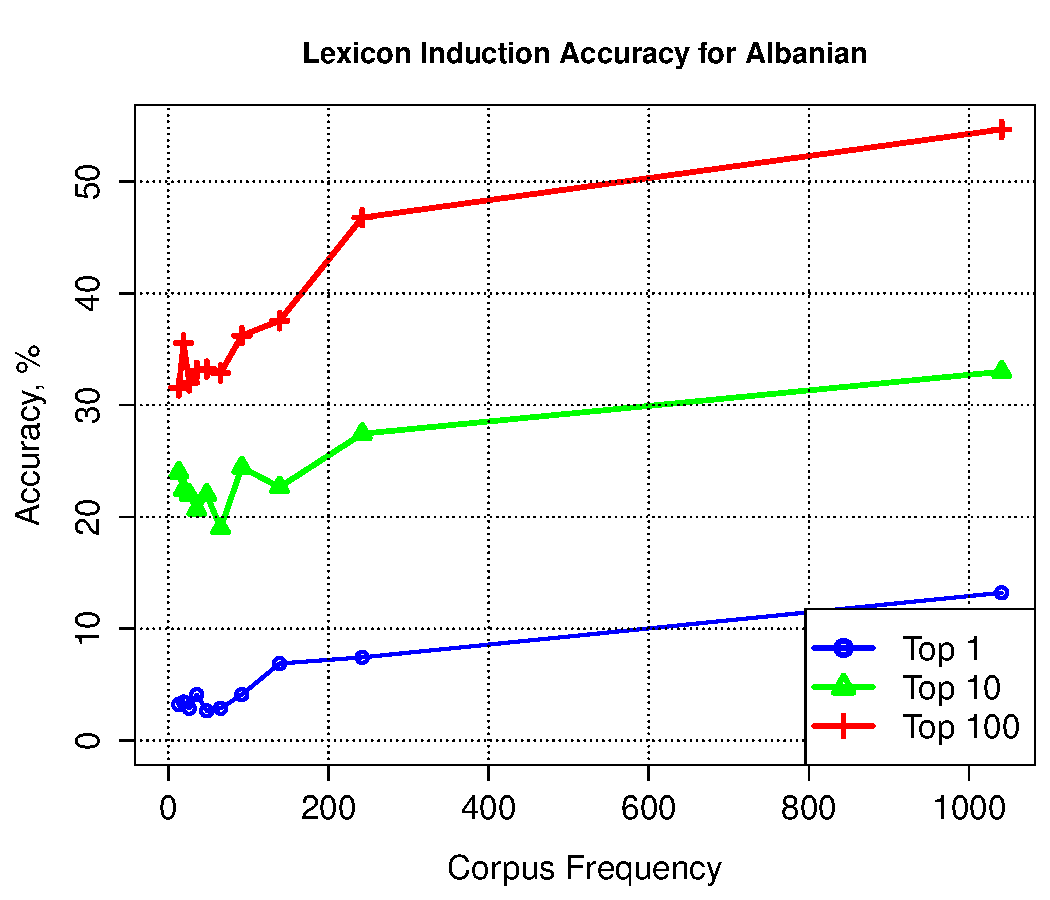
\includegraphics[width=0.9 \linewidth]{../byFreqGraphs/sq/lexinductnew.pdf}
\vskip -0.15in
\caption{Albanian bilingual lexicon induction results}
%\vskip -0.2in
\label{fig:bli.sq} 
\end{center}
\end{figure}

\begin{figure}
%\vskip 0.0in
\begin{center}
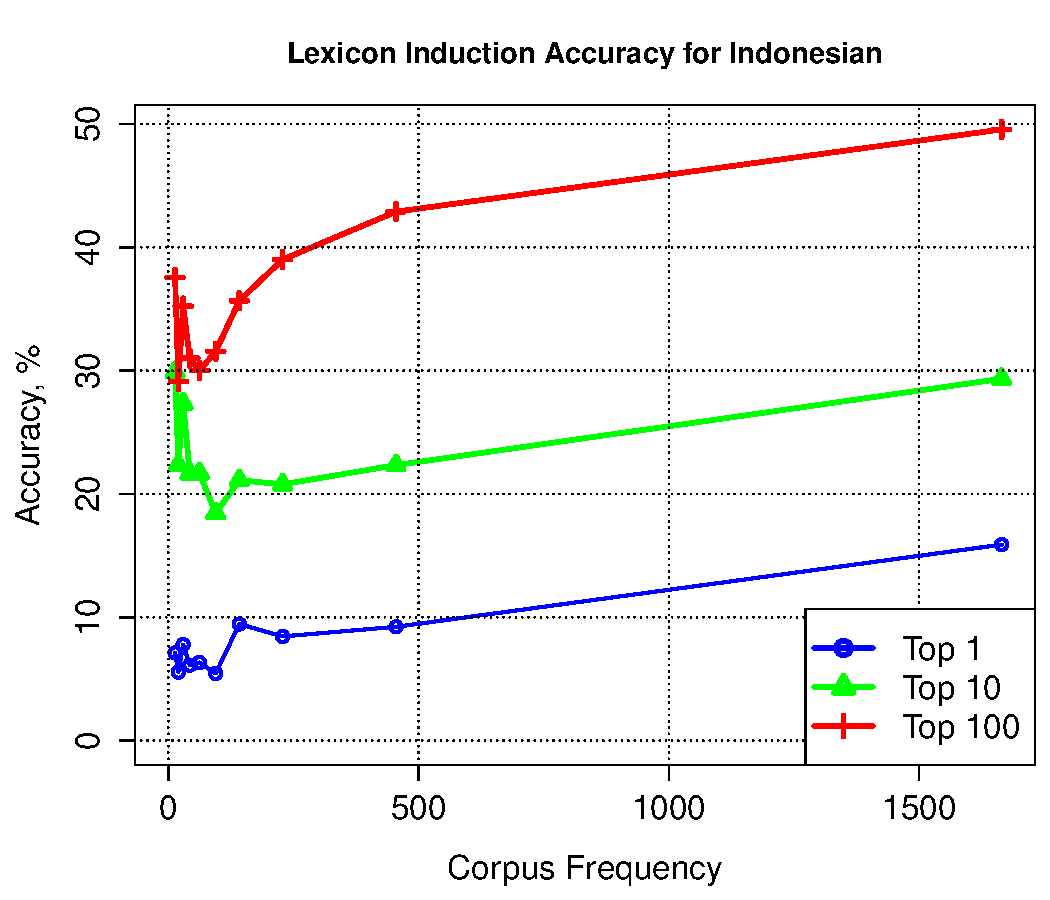
\includegraphics[width=0.9 \linewidth]{../byFreqGraphs/id/lexinductnew.pdf}
\vskip -0.15in
\caption{Indonesian bilingual lexicon induction results}
%\vskip -0.2in
\label{fig:bli.id} 
\end{center}
\end{figure}



\begin{figure}
%\vskip 0.0in
\begin{center}
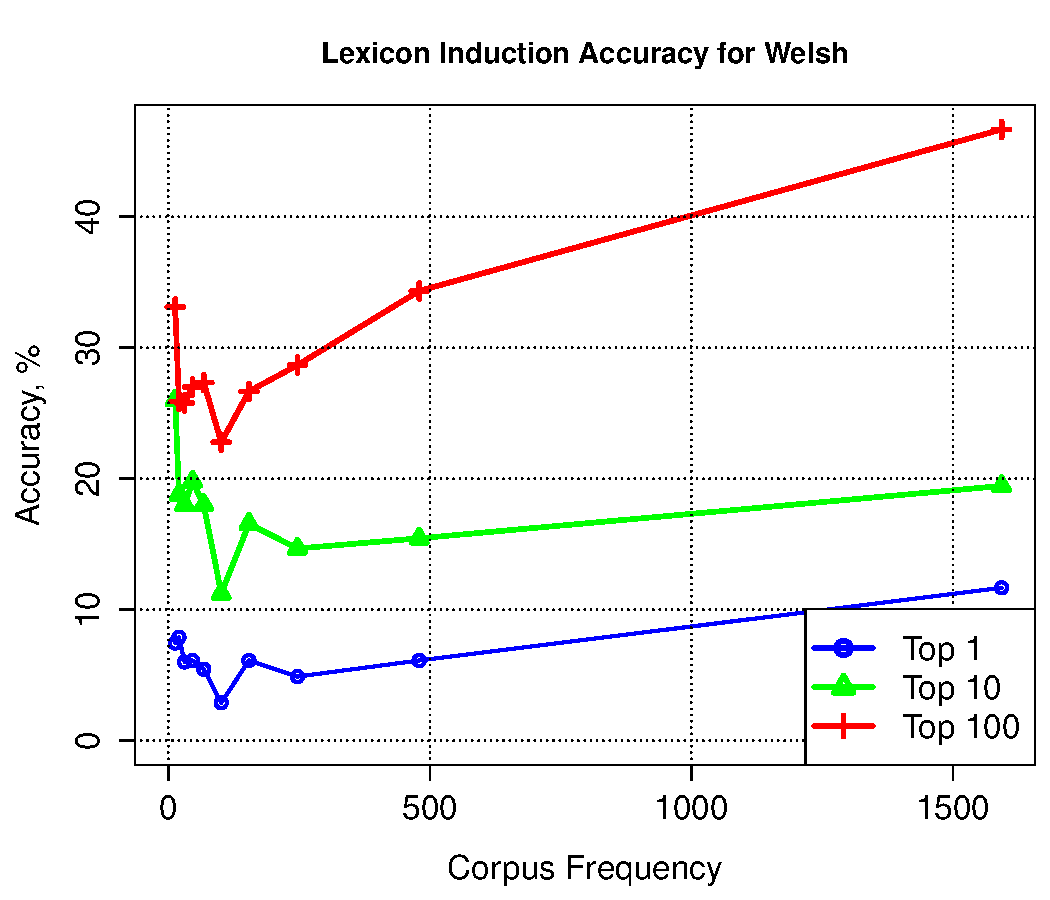
\includegraphics[width=0.9 \linewidth]{../byFreqGraphs/cy/lexinductnew.pdf}
\vskip -0.15in
\caption{Welsh bilingual lexicon induction results}
%\vskip -0.2in
\label{fig:bli.cy} 
\end{center}
\end{figure}



\begin{figure}
%\vskip 0.0in
\begin{center}
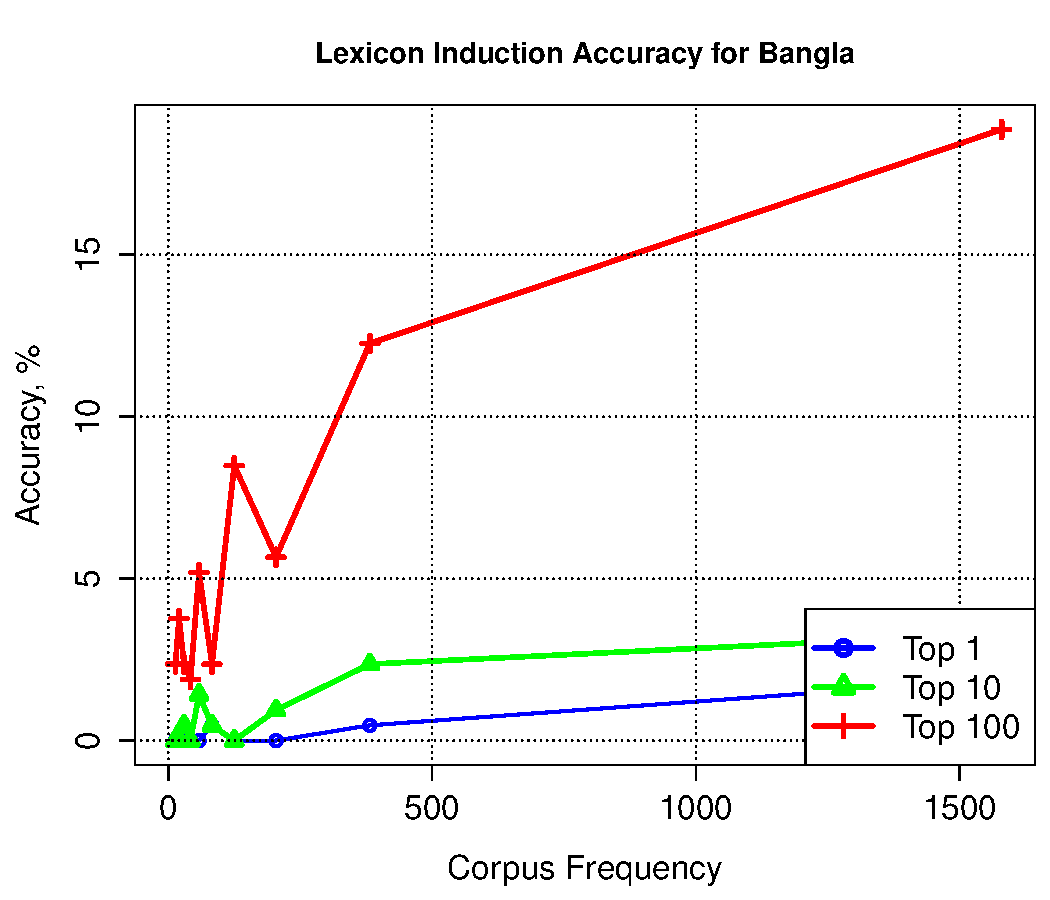
\includegraphics[width=0.9 \linewidth]{../byFreqGraphs/bn/lexinductnew.pdf}
\vskip -0.15in
\caption{Bengali bilingual lexicon induction results}
%\vskip -0.2in
\label{fig:bli.bn} 
\end{center}
\end{figure}

\begin{figure}
%\vskip 0.0in
\begin{center}
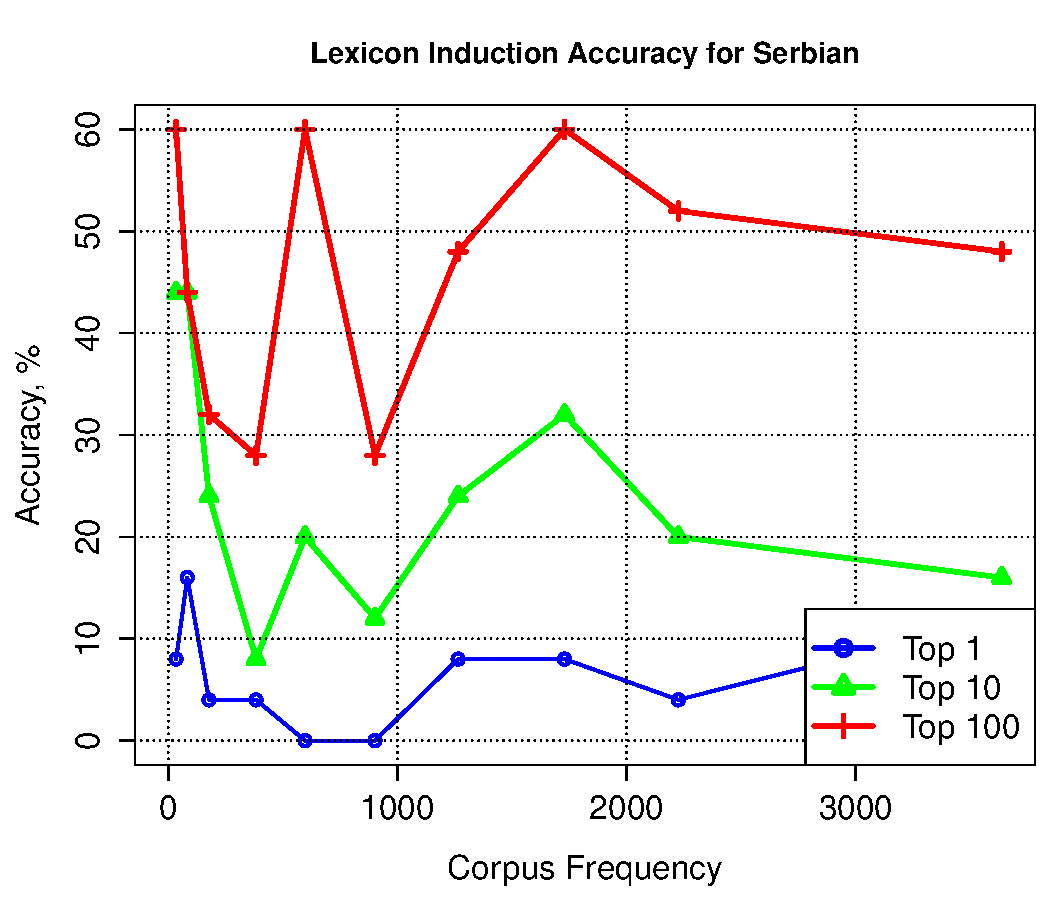
\includegraphics[width=0.9 \linewidth]{../byFreqGraphs/sr/lexinductnew.pdf}
\vskip -0.15in
\caption{Serbian bilingual lexicon induction results}
%\vskip -0.2in
\label{fig:bli.sr} 
\end{center}
\end{figure}

\clearpage

\begin{figure}
%\vskip 0.0in
\begin{center}
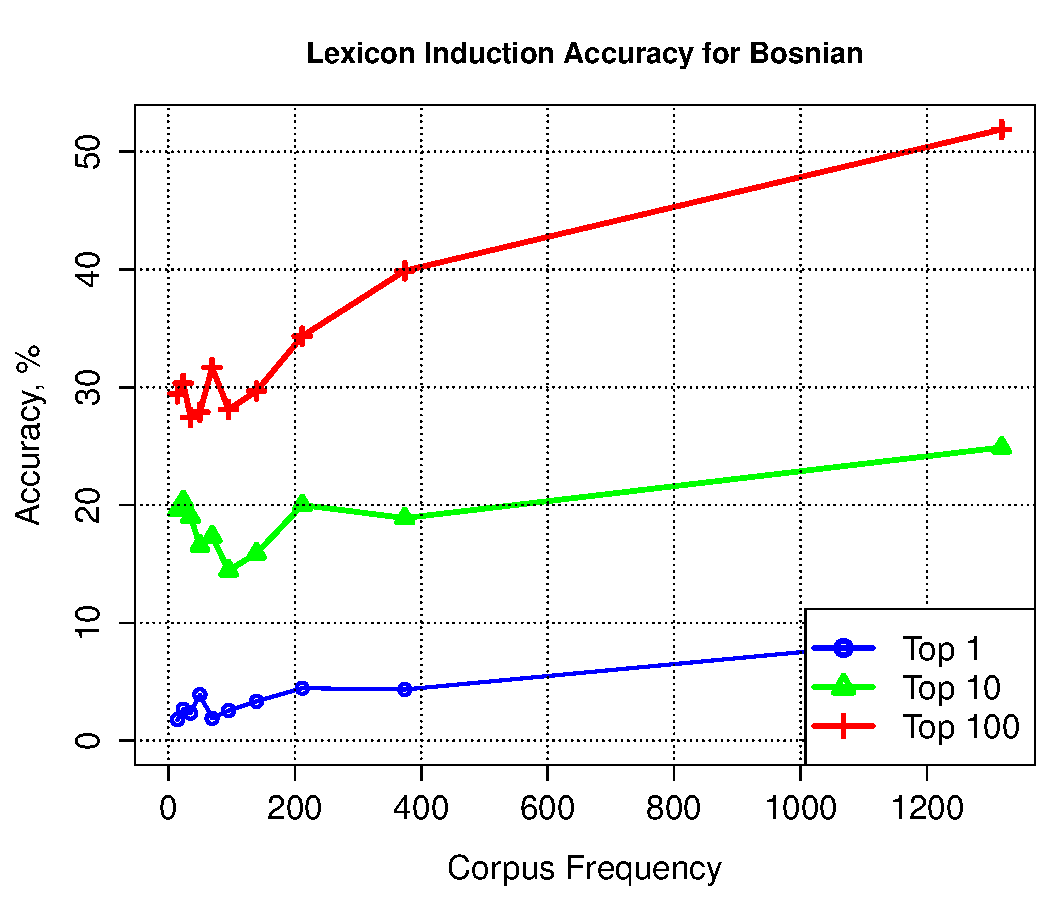
\includegraphics[width=0.9 \linewidth]{../byFreqGraphs/bs/lexinductnew.pdf}
\vskip -0.15in
\caption{Bosnian bilingual lexicon induction results}
%\vskip -0.2in
\label{fig:bli.bs} 
\end{center}
\end{figure}



\begin{figure}
%\vskip 0.0in
\begin{center}
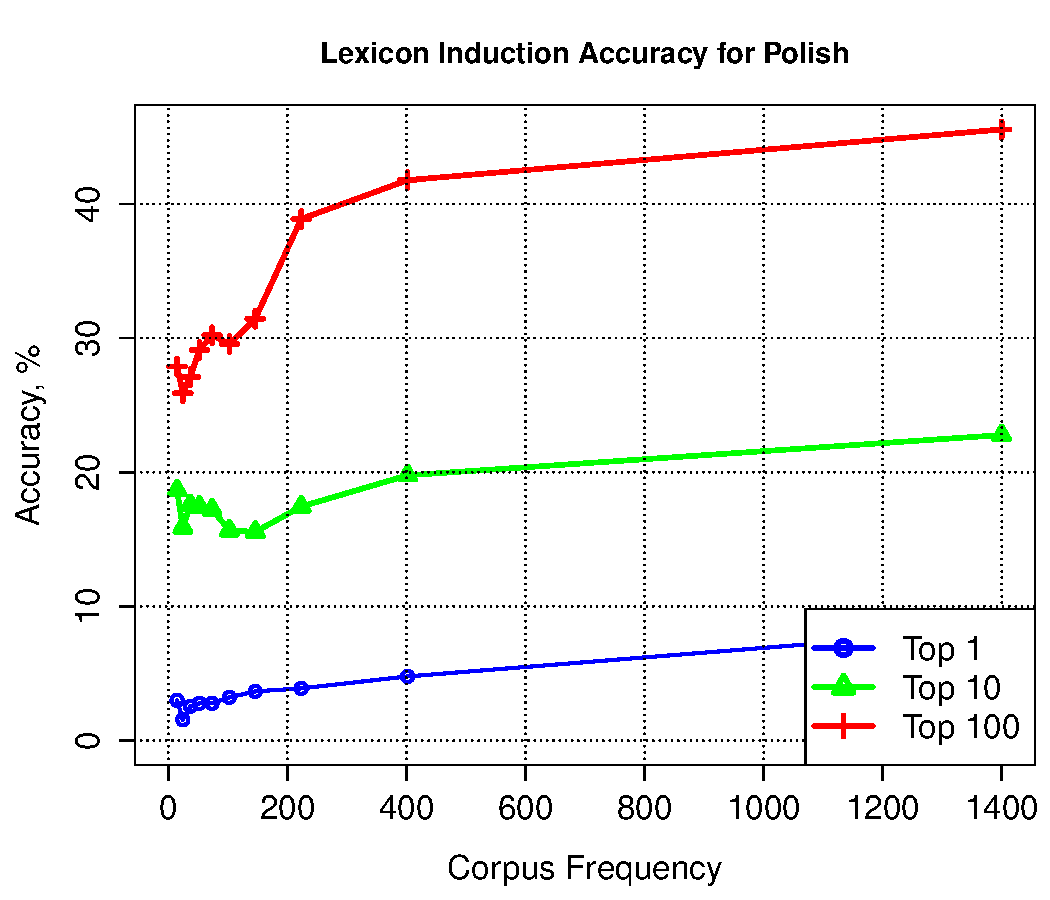
\includegraphics[width=0.9 \linewidth]{../byFreqGraphs/pl/lexinductnew.pdf}
\vskip -0.15in
\caption{Polish bilingual lexicon induction results}
%\vskip -0.2in
\label{fig:bli.pl} 
\end{center}
\end{figure}

\begin{figure}
%\vskip 0.0in
\begin{center}
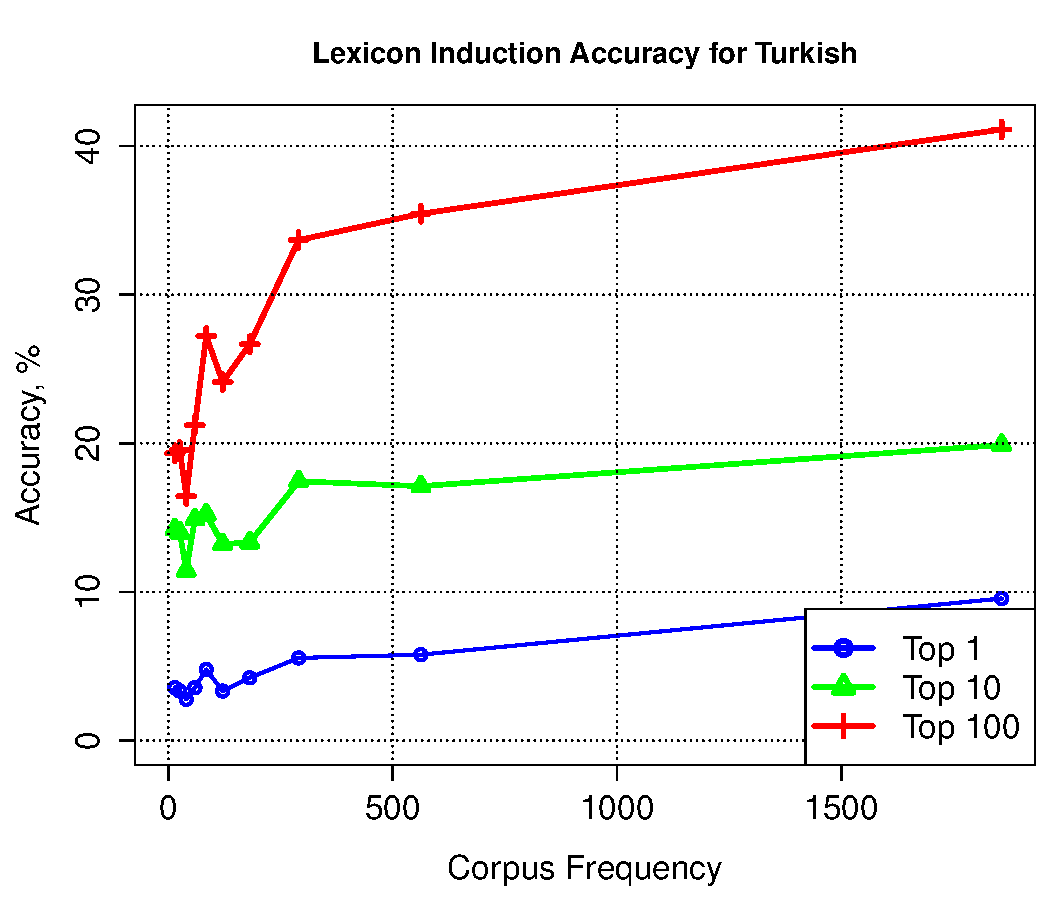
\includegraphics[width=0.9 \linewidth]{../byFreqGraphs/tr/lexinductnew.pdf}
\vskip -0.15in
\caption{Turkish bilingual lexicon induction results}
%\vskip -0.2in
\label{fig:bli.tr} 
\end{center}
\end{figure}



\begin{figure}
%\vskip 0.0in
\begin{center}
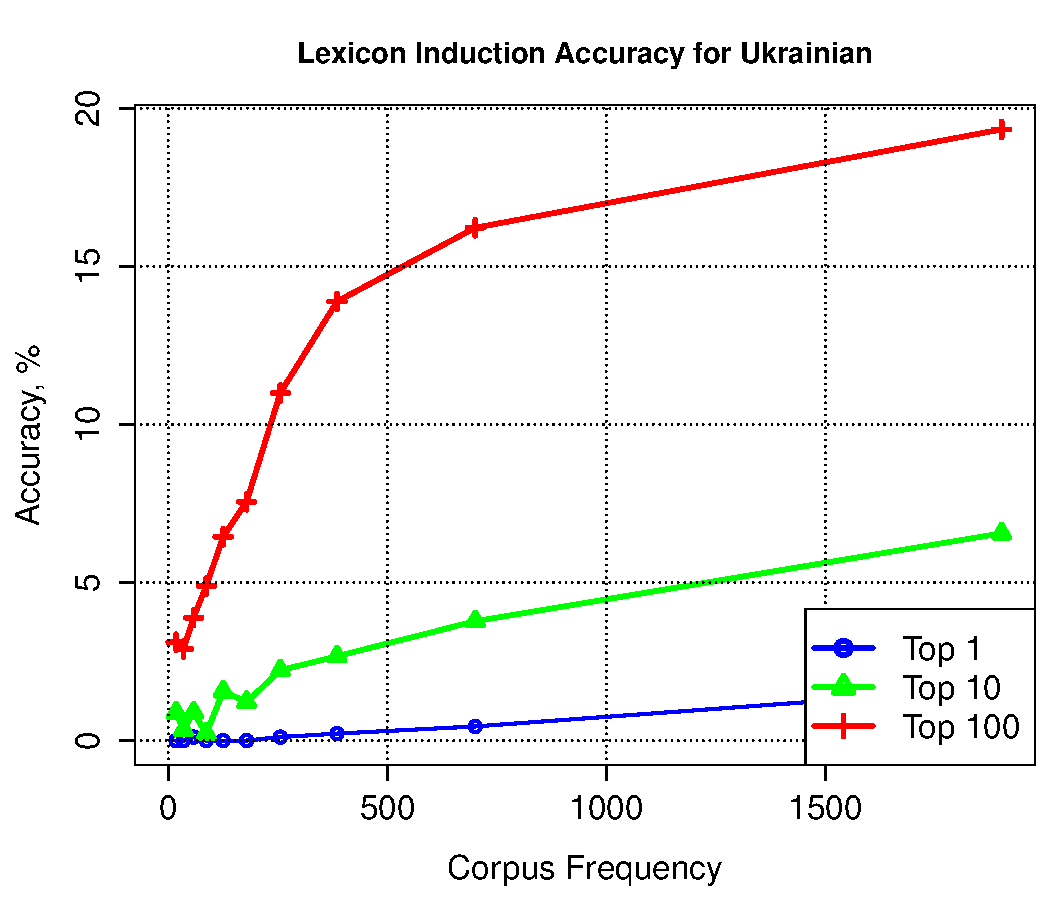
\includegraphics[width=0.9 \linewidth]{../byFreqGraphs/uk/lexinductnew.pdf}
\vskip -0.15in
\caption{Ukrainian bilingual lexicon induction results}
%\vskip -0.2in
\label{fig:bli.uk} 
\end{center}
\end{figure}


\begin{figure}
%\vskip 0.0in
\begin{center}
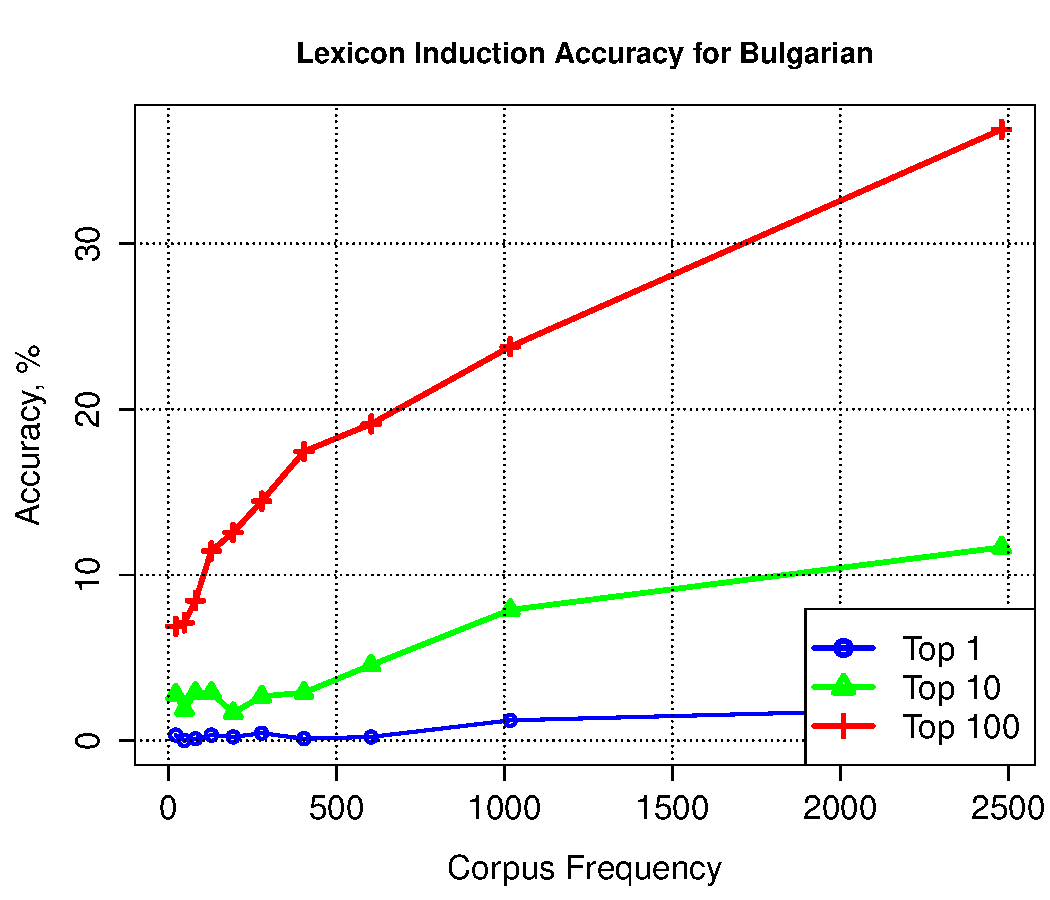
\includegraphics[width=0.9 \linewidth]{../byFreqGraphs/bg/lexinductnew.pdf}
\vskip -0.15in
\caption{Bulgarian bilingual lexicon induction results}
%\vskip -0.2in
\label{fig:bli.bg} 
\end{center}
\end{figure}

\begin{figure}
%\vskip 0.0in
\begin{center}
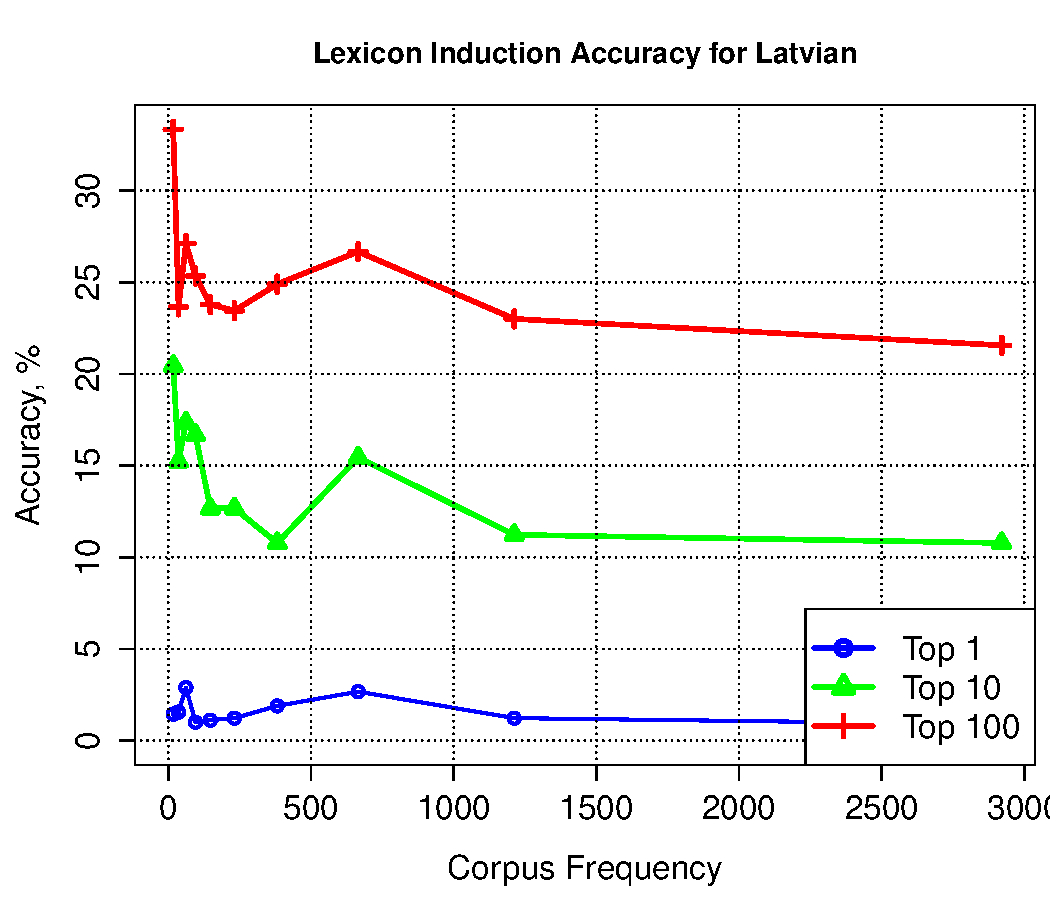
\includegraphics[width=0.9 \linewidth]{../byFreqGraphs/lv/lexinductnew.pdf}
\vskip -0.15in
\caption{Latvian bilingual lexicon induction results}
%\vskip -0.2in
\label{fig:bli.lv} 
\end{center}
\end{figure}

\clearpage


\begin{figure}
\vskip 0.0in
\begin{center}
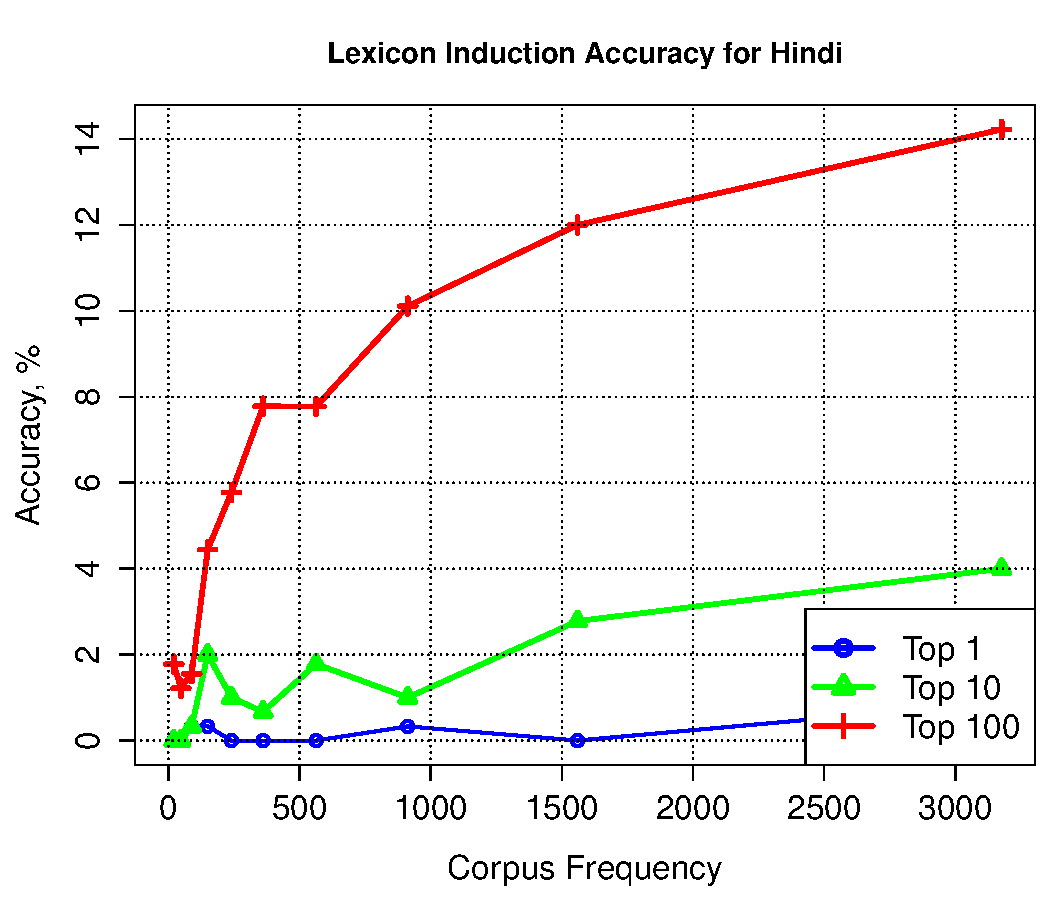
\includegraphics[width=0.9 \linewidth]{../byFreqGraphs/hi/lexinductnew.pdf}
\vskip -0.15in
\caption{Hindi bilingual lexicon induction results}
\vskip -0.2in
\label{fig:bli.hi} 
\end{center}
\end{figure}



\begin{figure}
\vskip 0.0in
\begin{center}
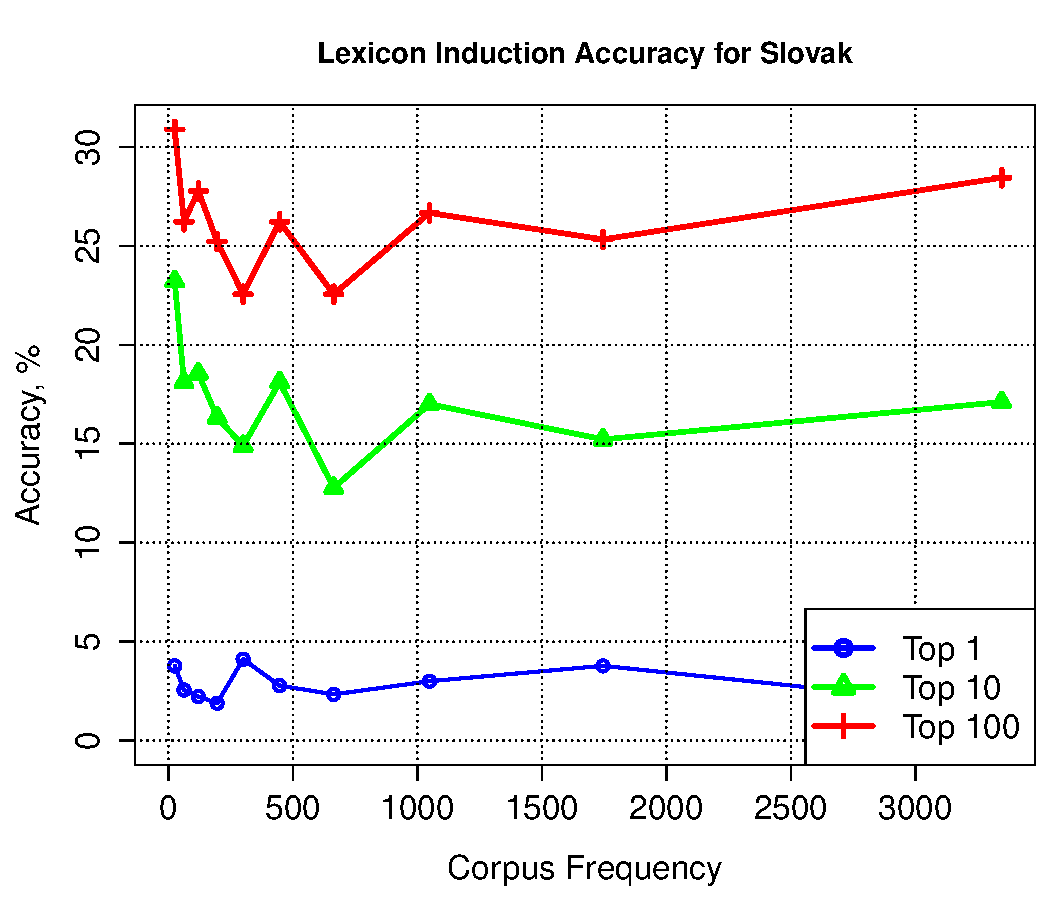
\includegraphics[width=0.9 \linewidth]{../byFreqGraphs/sk/lexinductnew.pdf}
\vskip -0.15in
\caption{Slovak bilingual lexicon induction results}
\vskip -0.2in
\label{fig:bli.sk} 
\end{center}
\end{figure}



%\begin{figure}
%\vskip 0.0in
%\begin{center}
%\includegraphics[width=0.9 \linewidth]{/Users/anni/Projects/unsup_translation/babelClean/LIMTresults/byFreqGraphs/ms/lexinductnew.pdf}
%\vskip -0.15in
%\caption{Malaysian bilingual lexicon induction results}
%\vskip -0.2in
%\label{fig:bli.ms} 
%\end{center}
%\end{figure}


%\newpage
%\clearpage



\section{Experiments 2: Machine translation without parallel data}\label{sec:mtwpd}
In the second set of experiments, we perform end-to-end machine translation, translating several Wikipedia pages in each of our 23 languages. We chose to translate the following source language Wikipedia pages because they are familiar topics, cover a variety of subjects, and exist in nearly all of our languages of interest: Barack Obama, New York, Computer, Islam, Forest. 

We generated phrase tables for each source language based on the dictionaries described in Section \ref{ssec:dicts} as well as induced translations for OOV words (source language words in the Wikipedia pages that do not have dictionary translations). We used the methods described in Section \ref{ssec:dicts} and our monolingual web crawl data to propose 50 translations for each OOV source language word.

Each phrase pair in the translation table is scored using each of the same similarity scores described in Section \ref{sec:lexinduc}; contextual and temporal similarity based on data from web crawls, and orthographic similarity. Additionally, we compute a contextual similarity score based on the Wikipedia monolingual data. Finally, we also compute a {\bf topic similarity} score for each phrase pair. To estimate this score, we gather topical signatures for each source and target language phrase. Topical signature vectors are the length of the number of interlingually linked Wikipedia pages in the source language and English Wikipedias and contain counts of how many times each phrase appeared on a given page. With the interlingual links, we are able to directly compute the similarity between these topic signatures. 

We don't have a bitext to use as a development set for tuning the feature weights, so we reuse the weights that were learned for a Spanish-English MT experiment involving exactly the same feature set. Of course, the source language and corpora change substantially in these new experiments, and the optimal weights are unlikely to be the same. In the future we hope to collect a few thousand sentences translations for each language, which would be enough to tune feature weights using, for example, MERT.

Because we do not have exact translations for each of our source language Wikipedia pages, we cannot evaluate translation quality with an automatic metric like BLEU. However, because the topics are familiar, it is possible to read the output and get a qualitative sense of the translation quality. Table \ref{table:qualtrans} shows the first few lines of each source language page on {\it Barack Obama} translated into English.

\onecolumn
%\begin{longtable*}\footnotesize
\begin{center}
\begin{longtable}{|p{1.5cm}|p{13cm}|}
\hline
%\multicolumn{2}{c}{ }\\
Language & Translation Output \\
\endfirsthead
\hline
Language & Translation Output \\
\endhead
\hline
Azeri & {barack hussein obama ( ing. barack hussein obama year ; 4 august 1961 ) - media the united states 44th president . 
in 2009 literary literary award substitute .  vital . 4 august 1961 hawaii in whether born the barack hussein gallery qarad?rili father ordinary also barack hussein obama ( father ) , a?d?rili his mother ordinary the stenli enn danhem was keniyadan the his father with kanzasdan being the mother hawaii university am were . barack obama in 1983 in colombia university graduated in 1985 and in chicago köç?r?k there and murder unemployment wrapped mehelle living conditions improve for the responsibility studying group work began . 1991 equipment in harvard right school he graduated from it and , d? harvard right communities magazine editor occurred first qarad?rili america .} \\
\hline
Nepali & {बराक हुसैन obama ( birth : 4 august , 1961 ) american ४४औं country is he this first country अश्वेत ( african अमरीकन ) country is । 20 he january , 2009 of national day position strengthening get done is । obama इलिनॉय राज्यबाट कनिष्ठ सेनेटर and 2008 in राष्टपति american sympathy for democratic party candidate । was obama हार्वर्ड ल स्कूलबाट san in 1991 graduate make , where he हार्वर्ड ल first रिव्यूका african अमरीकी also president was । 1997 from २००४ इलिनॉय सेनेटमा three complete सेवाकाल to do before obama community आयोजकको shape did work and citizens rights अधिवक्ताका shape did प्रेक्टिस 1992 from २००४ upto he शिकागो university law constitutional law adhyapaku also work did । san 2000 america in house आफ रिप्रेसेंटेटिवमा सीट do get unsuccessful after his january in 2003 sight अमरीकी सेनेटतर्फ was march in २००४ primary victory did receive and नवम्बर in 2003 सेनेटका for was elected}\\
\hline
Tamil & {பராக் உசேன் obama ( barack hussein obama , hatch : bəˈrɑːk hʊˈseɪn oʊˈbɑːmə , birth : august 4 , 1961 ) , american 2008 republic leader election win democratic party . candidates now he மேலவையிலும் இலினொய் state support young members . they are american history africa american race from first republic leader in power , and sent house fifth country native in power available for them . colombia university harvard clever but vain talk college degrees received obama politics world சேர்வதற்கு before chicago south in company joint ( community organizer ) public law worked lawyer . 1997இல் இலினொய் state legislature elected 2004 time was in office . 1992 first 2004 time chicago university clever but vain talk college professor worked .}\\
\hline
Somali & {barack obama it is man of also is you xargo and to many of usa years old it is 47 jir. the new the in region hawaii last month juli 27 teedii , year 1961 the dii. just birth father people of from black and he came wadaka kenya mother people and white and , of from watch kansas region of american and in him afadiisa intimacy obama , is have the two girls with called and with malia sasha the and his father the he left from him is two years old to education of the from give leads harvard. the after the dozens the to he returned land from of the he came kenya. aabbiihiis after , senator obama the mother is married man he came from the country indonesia to and then they have moved in the noolayeen while and in to in the one between 1969 until 1971dii. obama , the to immediately after , he returned hawaii region of mother is in indanusia , it was the where live the with parent mother new white was of .}\\
\hline
Uzbek & {barack hussein obama ii ( pronunciation : barack husayn obama launcher ; 1961-yili 4-avgust ) america 44- sham now president bungacha illinoys shtatining senatori fatherland accomplished .  2009-yil 9-oktabrida tinchlikka tries uchun specialized open prize taqdirini . source  ishoratlar  barack obama quo receiving obama maʼmuriyati , flighty. u n ' yu-y ' ork - american military qo ' mohammed shtatlardan biri. capital - albany citadel bellwether union ' seagulls on the 21st of august 1959 yilda kirgan , undan old - province of new york , then sovereign state in confederation .} \\
\hline
Romanian & {american interpreted remarks second speech ( in english / bəˈɹɑːk huˈseɪn oʊˈbɑːmə / ; b(born) . 4 august 1961 , honolulu , hawaii , son by american hussein obama , sr . — born at come from kenyană nyanza , from ethnicity luo — also al him ann dunham — born at wichita , kansas ) is al 44-lea president al states ( united first afro-american clear at this position ) , for parliamentary elections on 4 november 2008 , by joe cole as vice president ) . a former vest acting on 20 january 2009 but l-a changed by faking his george w. bush . son a kenyan , american hussein obama , sr. also al an american , ann dunham secretary , obama was game one important part was girl at honolulu , hawaii on six by decade was lived at jakarta , with mother and father of and cruel , indonesia release al liberal columbus also al proclamation from even by reprieve , above a stand that access into government and a state to join al senate state illinois between 1997 and 2004 , a director ago as fitting person , docent worldwide in particular and champion in rights protection civile.}\\
\hline
Albanian & {barack obama barack hussein obama ( born in 4 august 1961 in honolulu , barrack ) is president of 44-të of united states of to american barack obama is successful of price for nobel prize in year 2009. he is president first afro-american . in year 2004 he was elected to us senator in illinois. candidates like president for election campaign of and declared in 10 short 2007 in springfield ( unattached ) . on 3 june 2008 obama reached , according to data to tunnel , and offers necessary to votes for tag as to candidate for president , in that his party , left by after thus competition and us senator , wife of old to us president bill clinton in 27 august 2008 barack obama was ëmërua into way official to and from interior party demoktratike like candidate for president .} \\
\hline
Indonesian & {barack feared obama ii ( ; ) is american president union which currently served is american and president union which ke-44. barack served since 20 january 2009 replace george mandarin bush. before he is junior senator from illinois and then win in election president 2008 into 4 november 2008. into year 2009 , obama announced as winner gift act peace prize because promote international diplomacy to solve international problems . obama descent is africa first which served president union american after previously descent is africa the first farewell by a political parties large american to make president graduate and columbia university law school university ; harvard in there he served as president laws harvard reviewed , obama work as many coordinator and served as lawyer civil rights before making senate zlatko during three time begin 1997 until 2004.} \\
\hline
\caption{Translations of the first 4-5 sentences of each source language Wikipedia page on {\it Barack Obama}. Note that some characters in OOV words aren't displayed properly here. This table will be updated soon. In the meantime, these results can be found on the a01 clsp node, at: /mnt/data/anni/Experiments/LANG-en/work.3.dict/evaluation/plcw-m/test.tuned-filtered.out where LANG is the two character language code.} \label{table:qualtrans}  \\
\end{longtable}
\end{center}
%\vskip -0.1in
%\vskip -0.15in
%\end{longtable*}

\twocolumn

\section{Experiments 3: Monolingually-informed machine translation}

In the third set of experiments, we use the same techniques described above to translate source language documents for which we do have sentence-aligned English translations and, thus, are able to automatically score the output with the standard BLEU metric. In particular, we evaluate our methods on the Bengali, Tamil, and Hindi corpora released by \newcite{indianlangs}.

For each language, we perform end-to-end machine translation on the released test sets under the following conditions. In all cases we use a standard Moses phrase-based MT (PBMT) setup and vary only the source(s) of the phrase pairs contained in the phrase table and the set of features which are defined for each phrase pair.
\begin{enumerate}
\item{Phrase pairs extracted from bitext, bilingually estimated feature set, varying the amount of parallel training data.}
\item{Phrase pairs extracted from bitext, bilingually estimated feature set supplemented with full set of monolingual features (contextual-crawls, temporal-crawls, orthographic, contextual-wikipedia, topical-wikipedia), varying the amount of parallel training data. }
\item{Phrase table composed of dictionaries and induced translations for OOVs, full set of monolingual features.}
\item{Phrase pairs extracted from bitext supplemented with dictionaries and induced translations for OOVs, full bilingually and monolingually estimated feature set.}
\end{enumerate}
We use the development set for each language and MERT to tune our feature weights. We also compare our experimental results with those given in \newcite{indianlangs}, which compares Hiero and SAMT based grammars but does not experiment with a syntax-free phrasal grammar.

It should be noted that \newcite{indianlangs} uses a language model built from the target (English) side of the training data, rather than one built from a larger English corpus, such as the gigaword corpus. That work presents a boost of over a BLEU point when the smaller training-text based LM is used instead of a larger LM. We plan to experiment with the same smaller LM in the near future.

The results given in Figure \ref{fig:bntrans} are very encouraging. Our setup which uses all of the available parallel training data plus our dictionaries and induced translations for OOV words and both bilingually and monolingually estimated features (red line) outperforms all other setups, including the Heiro and SAMT-based experiments presented in \newcite{indianlangs}. Furthermore, supplementing the standard PBMT setup with monolingual features (blue line vs. green line) results in a consistent performance gain, across varying amounts of training data. The final thing to note is that using only our given and induced bilingual dictionaries and monolingual feature set to translate is equivalent to translating based on about $6,400$ training parallel sentences if the monolingual feature set is used (blue line) and about $8,000$ if the monolingual feature set isn't used (green line).

\begin{figure}
\vskip 0.0in
\begin{center}
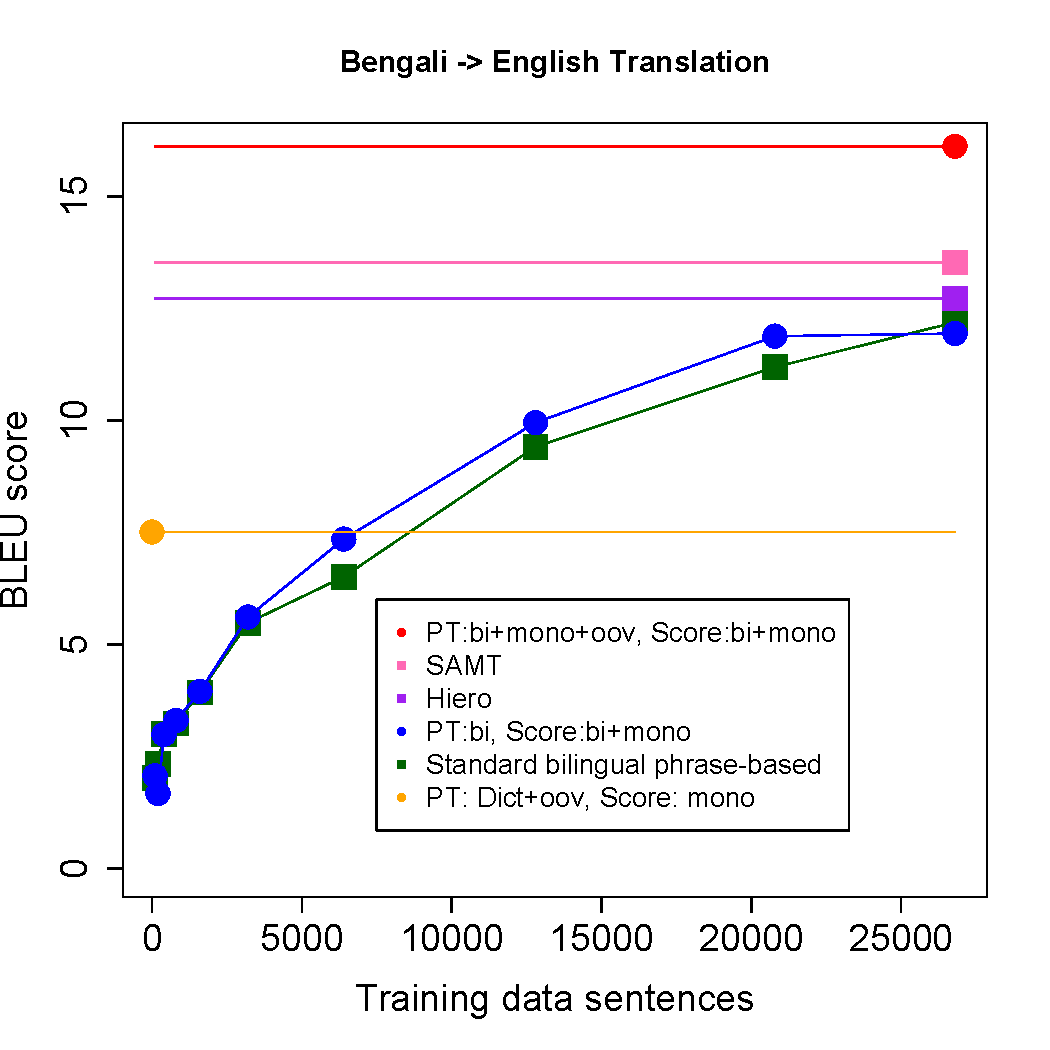
\includegraphics[width=1.05 \linewidth]{Figures/bntranslate.pdf}
\vskip -0.15in
\caption{End-to-end machine translation results for Bengali to English translation. It's noteworthy that the red line, which corresponds to our phrase-based system that uses the full available training data, our dictionaries, induced OOV translations and both bilingual and monolingual features outperforms all other experimental results.}
\vskip -0.2in
\label{fig:bntrans} 
\end{center}
\end{figure}

Unfortunately, these encouraging results aren't consistent across our Tamil and Hindi experiments. Figure \ref{fig:tatrans} shows the Tamil to English results. Here, both the Hiero and SAMT-based experiments presented in \newcite{indianlangs} outperform our full system, which uses our complete phrase table, with bilingually extracted phrase pairs and both bilingually and monolingually estimated features. Additionally, adding monolingual features doesn't seem to help performance. However, it is nice to note that using only our given and induced bilingual dictionaries and our monolingual feature set to translate is equivalent to translating with a PBMT system trained on about $16,000$ parallel sentences.

\begin{figure}
\vskip 0.0in
\begin{center}
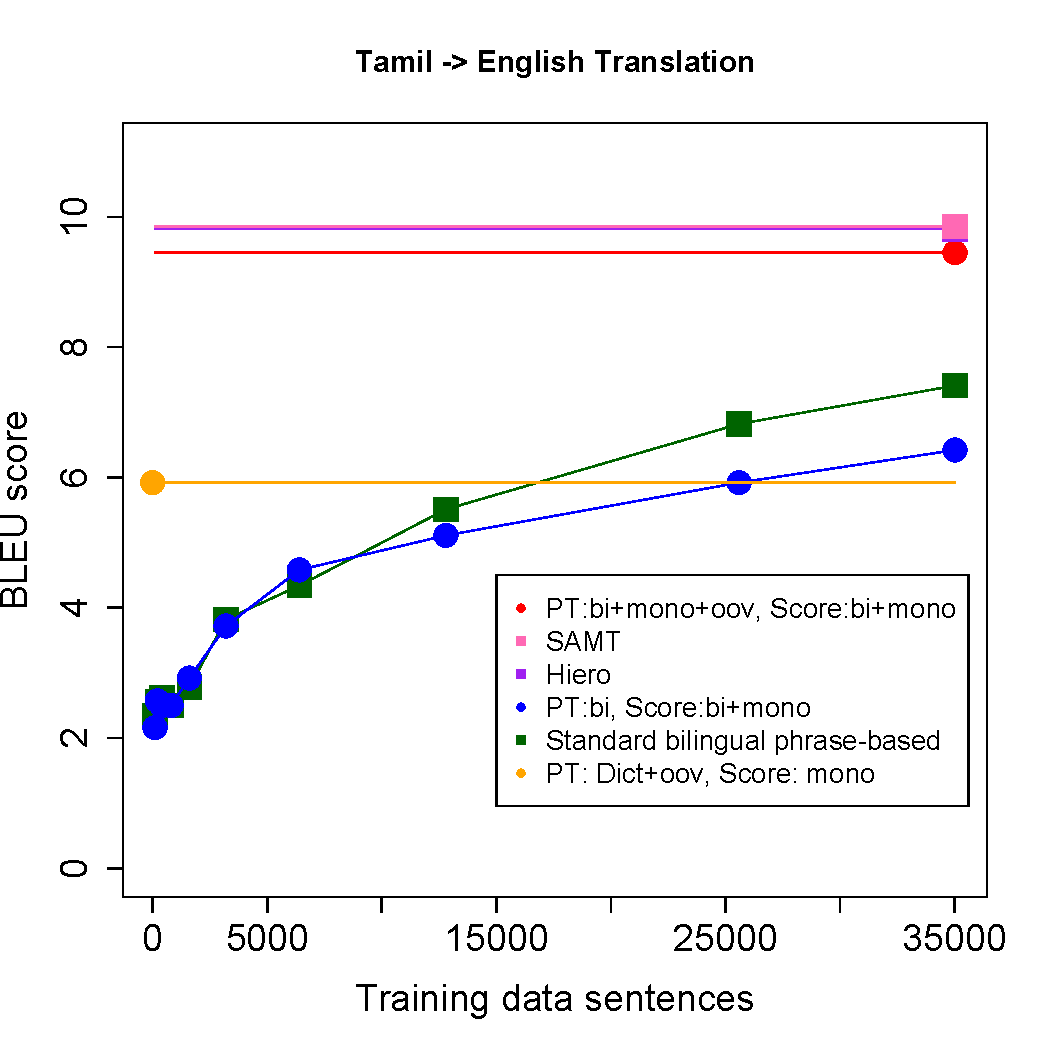
\includegraphics[width=1.05 \linewidth]{Figures/tatranslate.pdf}
\vskip -0.15in
\caption{End-to-end machine translation results for Tamil to English translation.}
\vskip -0.2in
\label{fig:tatrans} 
\end{center}
\end{figure}

\newpage

\bibliographystyle{naaclhlt2012}
\bibliography{limt}

\end{document}